\section{\proj{} Architecture Overview}

\begin{figure}[t]
    \centering
    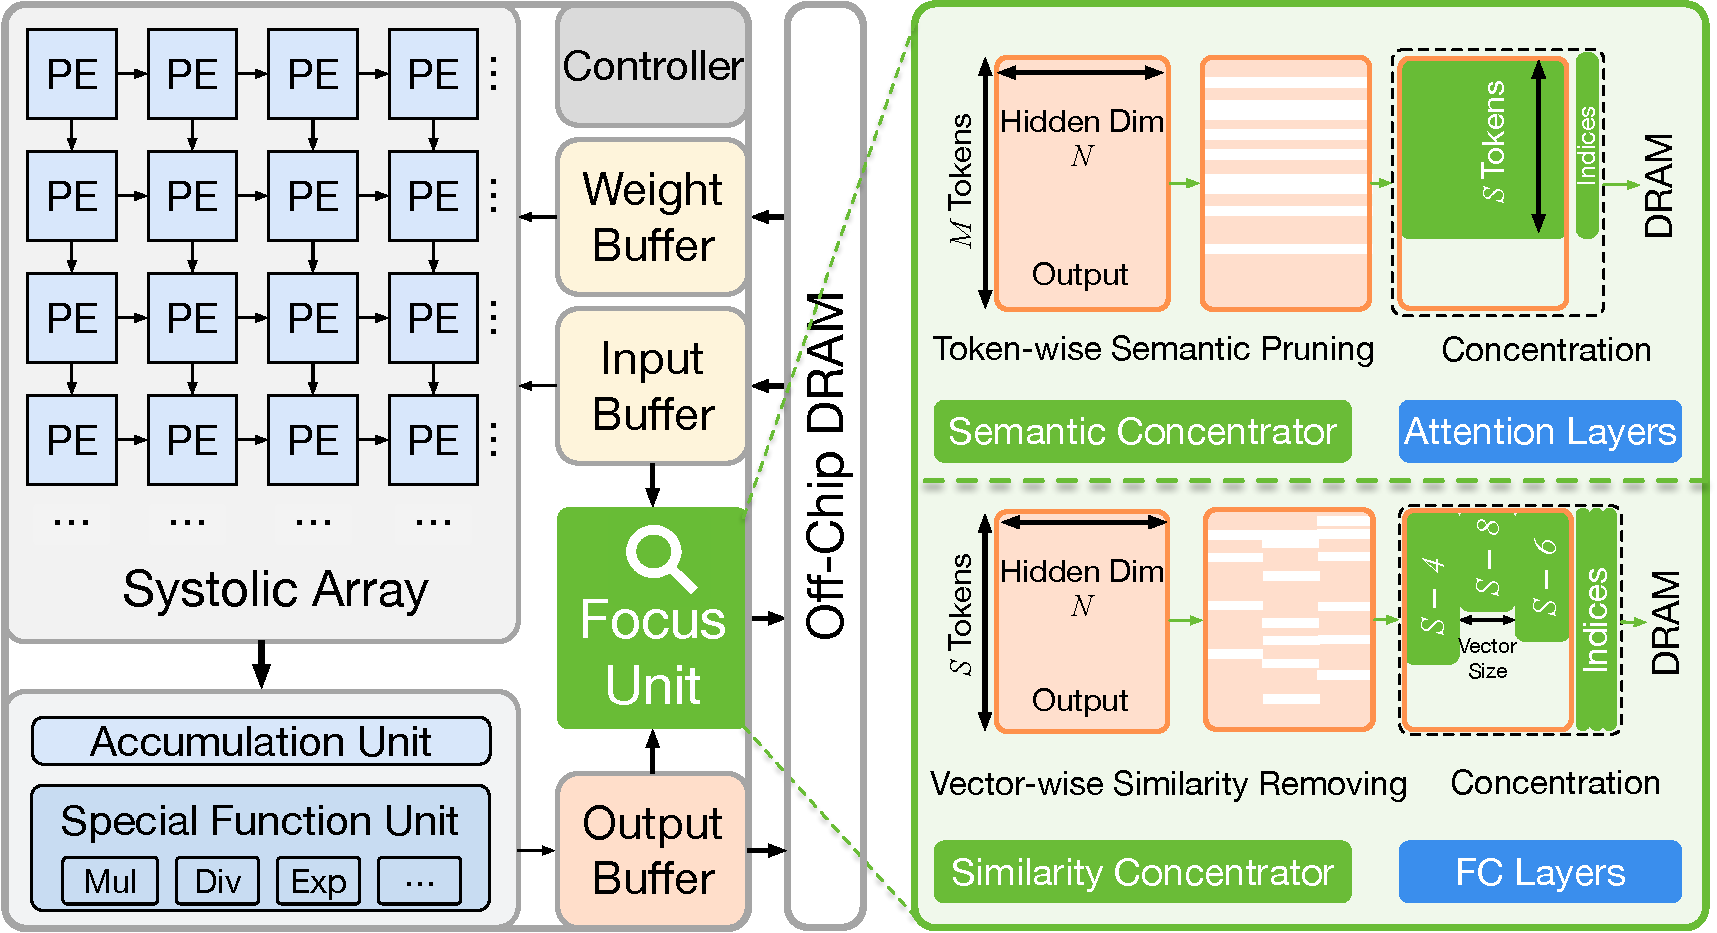
\includegraphics[width=\linewidth]{figure/overview.pdf}
    % \vspace{-6mm}
    \caption{Overview of the \proj{} architecture. 
    The \proj{} Unit integrates a Semantic Concentrator (SEC) and a Similarity Concentrator (SIC), positioned between compute stages to eliminate redundancy before memory write-back. Both modules operate in a streaming manner and run entirely on-chip.
    }
    \label{fig:focus_arch}
    % \vspace{-7mm}
\end{figure}

\proj{} introduces a modular \textbf{\proj{} Unit} to improve compute and memory efficiency in VLMs. 
As shown in \Fig{fig:focus_arch}, the \proj{} Unit is integrated near the memory interface of a standard systolic-array accelerator, intercepting data between compute stages without altering the core compute pipeline.
The \proj{} Unit consists of two streaming submodules:
\begin{itemize}
    \item \textbf{Semantic Concentrator (SEC)}: Performs token-level pruning in attention layers based on cross-modal Attention scores.
    \item \textbf{Similarity Concentrator (SIC)}: Performs vector-level redundancy elimination in fully connected (FC) layers, aligned with GEMM tiling.
\end{itemize}

\textbf{SEC} reduces the image token sequence length from $M$ to $S$.
It evaluates token importance using existing attention maps and prunes low-relevance tokens early in the pipeline.
Pruned tokens remain excluded in downstream layers, yielding cumulative savings in computation and memory access.

\textbf{SIC} further eliminates fine-grained redundancy among vectors within each GEMM tile.
It compares incoming vectors in a convolution-style window and replaces similar ones with index references to shared representatives.
This reduces the number of vectors processed per tile while preserving correctness via index-based reconstruction.

Both SEC and SIC operate entirely on-chip, support streaming dataflow, and dynamically adapt to data sparsity. 
By targeting complementary forms of redundancy from semantic and structural, \proj{} delivers efficient and scalable acceleration for Vision-Language Models.
We detail the hardware implementation of SEC and SIC in Sections~\ref{sec:sec} and~\ref{sec:sic}, respectively.